\documentclass[11pt]{book}
\usepackage[T1]{fontenc}
\usepackage{lmodern}
\usepackage{amsmath,amssymb,mathtools}
\usepackage[a4paper,margin=28mm]{geometry}
\usepackage{hyperref}
\usepackage{graphicx}
\usepackage{float}
\title{Informational Dynamics of Time}
\author{Adrian Lipa}
\date{2026}
\begin{document}
\maketitle
\chapter*{Abstract}
\addcontentsline{toc}{chapter}{Abstract}

This work develops a conditional research programme in which temporal structure is constructed from an explicitly declared relational model before spacetime geometry is introduced. The starting data are relational states and directed transitions carrying a normalized probability distribution, a normalized complex representative on phase-bearing sectors, positive transition weights, an ordering parameter distinct from metric clock time, and an inherited dimensionless normalization. The programme then asks which temporal quantities follow from those inputs by definition, exact identity, dynamical closure, or calibrated physical bridge.

Directed transitions carry both an exact Shannon entropy difference and a geometric phase link. Their combination with a separately typed non-exact path-affinity term is used to construct an auditable temporal transition phase, while closed-cycle identities separate exact state-function changes from genuinely non-exact directional information. Positive transition activity then generates an elapsed measure and a relative lapse before a spacetime metric is introduced. Downstream layers develop NOW support, bifurcation, transport, memory, constructive retrodiction, preregistered physical tests, and finally a temporal-to-spacetime closure interface.

The use of the word \emph{derived} is deliberately restricted: IDT does not claim that physical time follows uniquely from Shannon information alone. Its claims are conditional on the declared relational primitives and domains. Standard results from information theory, geometric phase, nonequilibrium response, quantum-state geometry, general relativity, and horizon thermodynamics are treated as imported background or recovery benchmarks rather than as new predictions.

Formal derivation, computational evidence, and physical claim status are maintained as separate layers. Exact identities, reference-model reconstructions, calibrated physical correspondences, and replicated measured results are not interchangeable evidence classes. The strongest present results are constructive and algebraic within their stated domains; the strongest physical claims remain attached to explicit falsification protocols whose calibration variables and null models are fixed independently of the measured outcome.

\chapter*{Methodological Note}
\addcontentsline{toc}{chapter}{Methodological Note}

The dependency rule of this programme is
\[
\boxed{\text{derive temporal structure first; introduce spacetime later}.}
\]
The construction begins from relational information and phase transport. Each new temporal object is admitted only after its upstream dependencies are explicit. The intended order is
\[
\begin{aligned}
\text{information}
&\to\text{directed transition}
\to\text{phase structure}
\to\text{temporal state}\\
&\to\text{NOW/bifurcation}
\to\text{transport/memory}
\to\text{metric calibration}\\
&\to\text{space}
\to\text{Einstein closure}.
\end{aligned}
\]

Mathematical construction, computational evidence, and physical claim status are kept distinct. A candidate is first assigned typed variables, equations, dependencies, and falsification conditions. Algebraic identities are proved where possible; numerical controls are used where analytic closure is not yet available. Only then can a claim move to a stronger registry status.

The ordering parameter used in the early formalism is kept distinct from metric clock time. Metric calibration is therefore a downstream bridge rather than a hidden starting assumption. Likewise, chirality, topology, fractal scaling, memory, and subjective temporal accumulation are treated as derived-property targets with their own observables and tests.

\section*{Prior-art and novelty discipline}

Whenever the construction invokes an established object, the corresponding chapter cites the standard source or a primary historical reference. Shannon entropy, Kullback--Leibler divergence, Pancharatnam/Berry phase, Onsager response, reversible Markov entropy gradients, Noether conservation, Einstein gravity, Bell/CHSH tests, and Hawking/Gibbons--Hawking horizon thermodynamics are therefore treated as external scientific context rather than as IDT discoveries.

A statement is called \emph{IDT-specific} only when it depends on the programme's own typed composition, decoder, activity measure, memory carrier, calibration map, or falsification rule. Recovery of a known physical equation is labelled a recovery benchmark. A physical discriminator requires an independently determined IDT quantity that can be evaluated before the target measurement is inspected.

\section*{Falsification before promotion}

For a proposed physical correspondence, the calibration map and null model must be fixed independently of the target outcome. If the same measured quantity is used both to define the IDT predictor and to confirm it, the exercise is classified as calibration or consistency checking rather than discrimination. Promotion to a physical result requires immutable raw data, uncertainty propagation, declared exclusions, and independent replication where the claim warrants it.

\tableofcontents
\chapter{Information and Relational Order}

The temporal programme begins from relational states rather than from a pre-existing time coordinate. Each state $s$ is assigned a probability distribution
\[
p(s)=(p_1,\ldots,p_m),
\qquad
p_i\geq0,
\qquad
\sum_i p_i=1,
\]
and its Shannon entropy in bits,
\[
\boxed{
H_S(s)=-\sum_i p_i(s)\log_2p_i(s).
}
\]
The inherited normalization is
\[
\kappa=\frac{\ln2}{24\pi}.
\]

For an admitted directed transition $e:a\to b$, the first informational quantity is the exact state-function difference
\[
\Delta H_e=H_S(b)-H_S(a).
\]
This quantity measures the change in the Shannon state entropy across that transition. Importantly, it is an exact difference. Therefore, for every closed directed cycle $C$,
\[
\boxed{
\sum_{e\in C}\Delta H_e=0.
}
\]
The identity follows by telescoping and has a direct methodological consequence: a state entropy difference can contribute to an open transition, but it cannot by itself generate a non-zero circulation around a closed cycle.

\section{Complex relational state and phase transport}

The same relational state is also represented by a normalized complex vector
\[
\psi(s)\in\mathbb C^m,
\qquad
\langle\psi|\psi\rangle=1.
\]
Whenever two consecutive states have non-zero overlap, define the normalized Pancharatnam link
\[
G_{a\to b}
=
\frac{\langle\psi_a|\psi_b\rangle}
{|\langle\psi_a|\psi_b\rangle|}
\in U(1).
\]
An open link is gauge-covariant under local rephasing of the state representatives. The ordered product of links around a closed cycle is gauge-invariant and defines the discrete geometric holonomy
\[
\gamma_B(C)
=
\operatorname{Arg}\!\left(\prod_{e\in C}G_e\right).
\]

\section{Shannon--phase transition link}

To connect informational change and phase transport without identifying them prematurely, introduce a transition-associated non-exact information increment $\sigma_e$. The first microscopic candidate closure is obtained from forward/reverse transition asymmetry. For strictly positive admitted transition probabilities,
\[
\boxed{
\sigma_{a\to b}
=
\log_2\frac{P(b\mid a)}{P(a\mid b)}.
}
\]
This quantity is path-level rather than a state entropy. It obeys $\sigma_{b\to a}=-\sigma_{a\to b}$ and vanishes for a symmetric transition pair. The candidate temporal link is
\[
\boxed{
L_e
=
G_e\exp\!\left[i\kappa\left(\Delta H_e+\sigma_e\right)\right].
}
\]
The corresponding transition phase weight is
\[
q_e=\operatorname{Arg}L_e.
\]
It can therefore enter the atomic temporal transition measure used later in the construction,
\[
\mathcal K_T=\sum_e q_e\,\delta_{s_e}.
\]

For a closed cycle the exact Shannon contribution cancels. Defining the cycle affinity
\[
\mathcal A_C
=
\sum_{e\in C}\sigma_e
=
\log_2\prod_{e\in C}
\frac{P_{e,+}}{P_{e,-}},
\]
gives
\[
\boxed{
\operatorname{Arg}\!\left(\prod_{e\in C}L_e\right)
=
\gamma_B(C)
+
\kappa\mathcal A_C
\pmod{2\pi}.
}
\]
This is the first structural separation in the derivation. The geometric part supplies phase holonomy. The exact Shannon state potential supplies open-transition information change. Directed path affinity supplies a non-exact information channel that can survive cycle closure.

A useful control follows immediately. If a strictly positive relational weight $\pi_s$ satisfies pairwise detailed balance,
\[
\pi_aP(b\mid a)=\pi_bP(a\mid b),
\]
then
\[
\sigma_{a\to b}=\log_2\frac{\pi_b}{\pi_a}
\]
and the cycle affinity telescopes to zero. Non-zero $\mathcal A_C$ is therefore a precise obstruction to this detailed-balance representation on the declared cycle.

The next derivational target is to determine how the relational density and viscosity fields modify the forward/reverse transition weights, rather than assigning those weights by hand.

\chapter{TIR Entrypoint}
The temporal branch imports only registry-declared TIR objects. Every downstream dependency is recorded explicitly so that the temporal derivation can be audited independently.

\chapter{Kähler Information Geometry}
The temporal construction begins on a state/information manifold \(\mathcal M\). Spacetime coordinates enter later at Einstein Closure.

\section{Relational forcing of the local geometry}
A positive context-sensitive internal elapsed measure has the local form
\[
 d\tau_{\rm int}=\phi(x,\lambda)\,d\lambda,
 \qquad \phi>0,
\]
so the scalar temporal pace is the Radon--Nikodym density of internal elapsed time with respect to the ordering parameter. In the current kinetic realization,
\[
\boxed{\phi=\frac{\mathfrak a}{\mathfrak a_\star}.}
\]

For a scalar informational functional \(\mathcal I\), the differential \(d\mathcal I\) is a covector. Coordinate-covariant local linear response therefore introduces a contravariant rank-two tensor \(G^{AB}\):
\[
V_I^A=-G^{AB}\partial_B\mathcal I.
\]
Positive informational descent makes the nondegenerate symmetric sector positive definite and defines
\[
g_{K,AB}=(G^{-1})_{AB}.
\]

A reversible phase response generated locally by \(\mathcal H_\alpha\) takes the form
\[
V_H^A=\Omega^{AB}\partial_B\mathcal H_\alpha,
\]
and preservation of \(\mathcal H_\alpha\) for arbitrary admitted phase covectors makes \(\Omega^{AB}\) antisymmetric. With the admitted unit \(U(1)\) phase generator \(J\),
\[
J^2=-I,
\qquad
\Omega^{AB}=J^A{}_{C}G^{CB},
\]
which yields the local exact-patch factorization
\[
\boxed{
\frac{dx}{d\lambda}
=-\operatorname{grad}_{g_K}\mathcal I
+J\operatorname{grad}_{g_K}\mathcal H_\alpha.
}
\]

\section{Global phase connection and holonomy}
The Shannon--Pancharatnam primitive assigns each admitted edge
\[
L_e=G_e\exp\!\left[i\kappa(\Delta H_e+\sigma_e)\right].
\]
Exact scalar differences obey \(\sum_C\Delta H_e=0\), while the closed-cycle temporal phase is
\[
\boxed{
\Phi_T(C)=\gamma_B(C)+\kappa\sum_{e\in C}\sigma_e\pmod{2\pi}.
}
\]
Admitted nonzero \(\Phi_T\) is therefore carried globally by the temporal \(U(1)\) connection and its holonomy. The scalar \(\mathcal H_\alpha\) remains the local generator on an exact patch; the connection supplies the transition and cycle data needed to patch those local descriptions across the state bundle.

The associated two-form is
\[
\omega(X,Y)=g_K(JX,Y).
\]
The complex-projective/Fubini--Study sectors used by the Memory construction supply an integrable complex structure, while the admitted Berry-curvature sector supplies a closed phase two-form. The resulting package
\[
\boxed{(\mathcal M,J,g_K,\omega)}
\]
is Kähler under these declared compatibility and closure conditions.

For an oriented two-chain \(\Sigma\), the signed Kähler-area diagnostic
\[
\mathcal A_K[\Sigma]=\int_\Sigma\omega
\]
obeys
\[
\mathcal A_K[-\Sigma]=-\mathcal A_K[\Sigma].
\]
This gives the formalism an orientation-sensitive geometric object. Temporal chirality is then tested downstream by the dynamics and holonomy gates.

\section{Visual phase portrait}
Figure~\ref{fig:kahler-flow-2d} gives a 2D slice of the Kähler time flow: informational descent provides the inward tendency, while the phase lift bends trajectories while preserving the typed separation of the two response channels.
\begin{figure}[H]
  \centering
  \includegraphics[width=0.78\textwidth]{figures/kahler_flow_2d.png}
  \caption{Two-dimensional Kähler time flow with contour levels of the informational functional and representative trajectories.}
  \label{fig:kahler-flow-2d}
\end{figure}

\chapter{Tensor--Scalar Temporal Field}
The temporal configuration is represented by a scalar pace together with a rank-two relational response sector. The scalar component is typed by the internal elapsed density
\[
\boxed{
\phi
=\frac{d\tau_{\rm int}}{d\lambda}
=\frac{\mathfrak a}{\mathfrak a_\star}>0.
}
\]
For the same ordering increment \(d\lambda\), distinct admitted relational states may therefore realize distinct internal elapsed increments.

The tensorial response is written locally as
\[
\boxed{
\mathcal R^{AB}=G^{AB}+\Omega^{AB},
}
\]
where
\[
G^{AB}=G^{BA},
\qquad
\Omega^{AB}=-\Omega^{BA}.
\]
The symmetric positive sector maps the informational covector to dissipative state transport,
\[
V_I^A=-G^{AB}\partial_B\mathcal I,
\]
while the antisymmetric sector maps a local exact phase covector to reversible state transport,
\[
V_H^A=\Omega^{AB}\partial_B\mathcal H_\alpha.
\]

Formalism 01C supplies the stationary Shannon informational scalar
\[
\boxed{
\mathcal I_\pi[p]=D_{\rm KL}^{(2)}(p\|\pi).
}
\]
For admitted stationary transition dynamics this scalar contracts. In the detailed-balance sector, Formalism 01D derives the exact symmetric response
\[
\boxed{
G^{(2)}_\pi(p)
=(\ln2)D^\top\operatorname{diag}[c_{ab}\Lambda(r_a,r_b)]D,
\qquad
r_a=\frac{p_a}{\pi_a},
}
\]
and the exact flow identity
\[
\boxed{
\dot p=-G^{(2)}_\pi(p)\nabla_p\mathcal I_\pi.
}
\]
The mass-conservation direction satisfies
\[
G^{(2)}_\pi\mathbf1=0,
\]
so the corresponding metric response is taken on the active simplex tangent quotient. At uniform zero-drive equilibrium,
\[
\boxed{
G^{(2)}_u(u)=\frac{\ln2}{m}K_0,
}
\]
which ties the symmetric information-response tensor directly to the relational-mobility Laplacian used by Temporal Wave.

In the admitted Kähler factorization on a compatible active sector,
\[
g_{K,AB}=(G^{-1})_{AB},
\qquad
\Omega^{AB}=J^A{}_{C}G^{CB},
\]
where the inverse is understood on the nondegenerate tangent sector when conservation constraints are present. On an exact phase patch the evolution law is
\[
\boxed{
\frac{dx}{d\lambda}
=-\operatorname{grad}_{g_K}\mathcal I
+J\operatorname{grad}_{g_K}\mathcal H_\alpha.
}
\]
This form is the coordinate-covariant factorization of the symmetric informational-response channel and the antisymmetric local phase-response channel established in Formalism 01A.

Formalism 01B supplies the global phase completion. The edge link
\[
L_e=G_e\exp\!\left[i\kappa(\Delta H_e+\sigma_e)\right]
\]
defines a temporal connection class whose closed-cycle holonomy is
\[
\boxed{
\Phi_T(C)=\gamma_B(C)+\kappa\sum_{e\in C}\sigma_e\pmod{2\pi}.
}
\]
The exact Shannon part telescopes on a closed cycle. Berry holonomy and non-exact affinity provide the global connection data. Thus \(\mathcal H_\alpha\) is typed as a local exact-patch generator, while the U(1) connection carries global phase patching and cycle information.

The tensor--scalar temporal architecture is therefore summarized locally by
\[
\boxed{
\mathcal T
=\bigl(\phi,\mathcal R^{AB}\bigr),
\qquad
\phi=\frac{\mathfrak a}{\mathfrak a_\star},
\qquad
\mathcal R^{AB}=G^{AB}+J^A{}_{C}G^{CB},
}
\]
with a global phase-connection layer supplying the holonomy class. The scalar answers how much internal elapsed time is realized per ordering increment. The symmetric tensorial sector has a Shannon--Onsager realization in probability coordinates, while the antisymmetric/connection sector carries orientation and circulation.

The next upstream task is to extend the response decomposition to stationary nonreversible dynamics while retaining the 01C relative-information contraction and the 01B connection/current structure. Downstream realizations are tested through Temporal Wave, NOW, Bifurcation, Transport, Memory and Retrodiction.

\section{nD slices of the tensor--scalar field}
Because the full tensor--scalar state lives in a space of dimension higher than two, Figure~\ref{fig:nd-slices} provides four schematic two-dimensional slices as a readable proxy for the richer field geometry.
\begin{figure}[H]
  \centering
  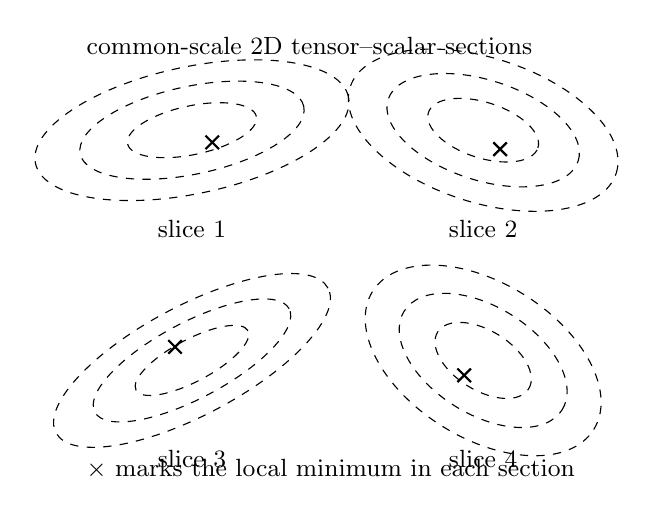
\begin{tikzpicture}[scale=0.86]
    \foreach \x/\y/\ang/\sx/\sy/\mx/\my/\lab in {
      -3.3/2.0/12/1.35/0.72/-3.0/1.82/{slice 1},
       1.0/2.0/-18/1.18/0.82/1.25/1.72/{slice 2},
      -3.3/-1.4/28/1.30/0.62/-3.55/-1.20/{slice 3},
       1.0/-1.4/-32/1.10/0.88/0.72/-1.62/{slice 4}}
    {
      \begin{scope}[shift={(\x,\y)},rotate=\ang]
        \draw[dashed] (0,0) ellipse ({1.75*\sx} and {1.30*\sy});
        \draw[dashed] (0,0) ellipse ({1.25*\sx} and {0.90*\sy});
        \draw[dashed] (0,0) ellipse ({0.72*\sx} and {0.50*\sy});
      \end{scope}
      \draw[thick] (\mx-0.10,\my-0.10) -- (\mx+0.10,\my+0.10);
      \draw[thick] (\mx-0.10,\my+0.10) -- (\mx+0.10,\my-0.10);
      \node[font=\small] at (\x,\y-1.45) {\lab};
    }
    \node[font=\small,anchor=west] at (-5.0,3.25) {common-scale 2D tensor--scalar sections};
    \node[font=\small,anchor=west] at (-5.0,-3.0) {$\times$ marks the local minimum in each section};
  \end{tikzpicture}
  \caption{Schematic four common-scale two-dimensional slices of a higher-dimensional tensor--scalar surrogate. The fixed tensor coordinates deform the local informational landscape; the cross marks the minimum in each slice.}
  \label{fig:nd-slices}
\end{figure}

\chapter[Chiral--Fractal Temporal Topology]{Chiral--Fractal Temporal Topology as a Derived-Property Gate}
The Neutrinotime line motivates a fractal--chiral temporal topology as a comparison target. In the present derivation, the target is decomposed into independently testable quantities:
\[
I_{\rm top}[\Gamma],\qquad \chi[\Gamma],\qquad D_F[\Gamma].
\]
These denote, respectively, a topological invariant, a signed chirality/orientation observable, and a fractal-scaling observable of an orbit or invariant set \(\Gamma\).

A minimal chirality candidate is a signed holonomy,
\[
\chi[C]=\operatorname{sgn}\!\left(\oint_C A\right),
\]
whenever the dynamical state bundle supplies an admitted connection \(A\). Orientation reversal must reverse the sign of \(\chi\) while declared non-chiral invariants remain unchanged.

Fractality is measured prospectively from the derived tensor--scalar dynamics through \(D_F\), a renormalization relation, a Lyapunov diagnostic, or another explicit scaling test. A linear Kähler control supplies the non-fractal reference class.

The relation between event-localized NOW and a dynamical bifurcation locus remains an open bridge. They are maintained as separate typed objects until an equivalence theorem or prospective experiment closes that dependency.

\section{Visual intuition for chirality and event structure}
The schematic rendering in Figure~\ref{fig:temporal-ribbon-3d} shows a single trajectory lifted over an informational landscape, making visible the joint role of orbital phase and informational descent. Figure~\ref{fig:event-measure} then shows a schematic discrete event measure extracted from an evolving informational signal.
\begin{figure}[H]
  \centering
  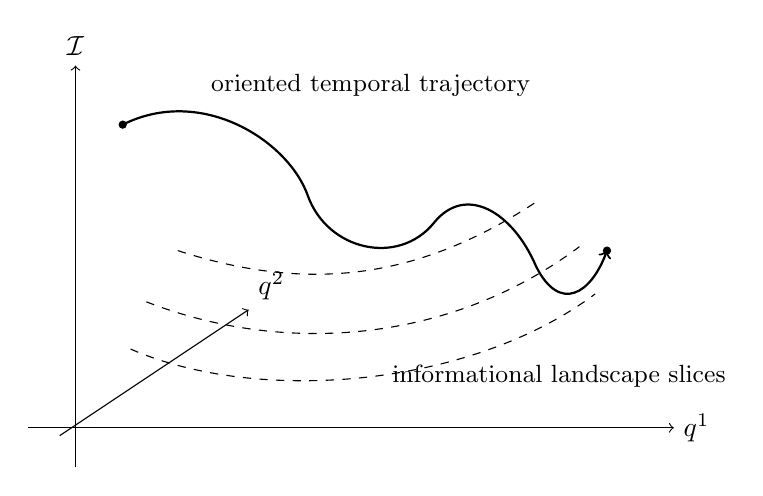
\begin{tikzpicture}[scale=1.0]
    \draw[->] (-4.0,-1.9) -- (4.2,-1.9) node[right] {$q^1$};
    \draw[->] (-3.4,-2.4) -- (-3.4,2.7) node[above] {$\mathcal I$};
    \draw[->] (-3.6,-2.0) -- (-1.2,-0.4) node[above right] {$q^2$};
    \draw[dashed] (-2.7,-0.9) .. controls (-1.1,-1.6) and (1.6,-1.4) .. (3.2,-0.2);
    \draw[dashed] (-2.5,-0.3) .. controls (-0.7,-1.0) and (1.4,-0.8) .. (3.0,0.4);
    \draw[dashed] (-2.1,0.35) .. controls (-0.4,-0.2) and (1.0,0.0) .. (2.5,1.0);
    \draw[->,thick]
      (-2.8,1.95)
      .. controls (-1.8,2.45) and (-0.7,1.75) .. (-0.45,1.05)
      .. controls (-0.20,0.35) and (0.70,0.15) .. (1.15,0.70)
      .. controls (1.55,1.20) and (2.15,0.85) .. (2.45,0.15)
      .. controls (2.75,-0.45) and (3.15,-0.20) .. (3.35,0.35);
    \fill (-2.8,1.95) circle (1.5pt);
    \fill (3.35,0.35) circle (1.5pt);
    \node[font=\small,anchor=west] at (-1.8,2.45) {oriented temporal trajectory};
    \node[font=\small,anchor=west] at (0.5,-1.25) {informational landscape slices};
  \end{tikzpicture}
  \caption{Schematic lifted slice of temporal evolution on the Kähler informational landscape. The vertical coordinate represents the informational functional $\mathcal{I}$ along an oriented trajectory.}
  \label{fig:temporal-ribbon-3d}
\end{figure}
\begin{figure}[H]
  \centering
  \begin{tikzpicture}[x=0.92cm,y=1.0cm]
    \draw[->] (0,0) -- (11.2,0) node[right] {$\lambda$};
    \draw[->] (0,-0.2) -- (0,3.0) node[above] {event weight};
    \draw[dashed] (0,1.0) -- (10.7,1.0) node[right,font=\small] {reference level};
    \foreach \x/\h in {0.7/0.35,1.5/0.75,2.4/0.45,3.2/1.55,4.0/0.65,5.1/2.35,6.0/0.55,6.9/1.25,7.8/0.50,8.9/1.90,9.8/0.70}
      \draw[thick] (\x,0) -- (\x,\h);
    \foreach \x/\h in {3.2/1.55,5.1/2.35,6.9/1.25,8.9/1.90}
      \fill (\x,\h) circle (1.8pt);
    \node[font=\small,anchor=west] at (3.35,2.65) {localized event support};
  \end{tikzpicture}
  \caption{Schematic discrete event measure on the ordering parameter. Selected localized peaks illustrate the event-support coordinate used to compare temporal evolution with NOW localization.}
  \label{fig:event-measure}
\end{figure}

\chapter{Nature of the Temporal State}

The temporal architecture developed in this work is organized around an ordered relational support, a state carried on that support, directed event activity, transport between event surfaces, local bifurcation at admitted events, an internal elapsed measure, and retained memory lineage. These objects are typed separately and are joined by the dependency structure developed in the preceding and subsequent formal layers.

\section{Ordered relational support}

Let
\[
(S,\prec)
\]
be an ordered relational domain and
\[
\boxed{\Psi:S\to\mathcal H}
\]
the temporal-state map. The relation $\prec$ supplies precedence between admitted events, while $\Psi$ supplies the state assigned to the ordered support.

For an admitted transition $a\to b$, the directed kinetic representation is
\[
W_{a\to b}=M_{ab}e^{A_{ab}/2},
\qquad
W_{b\to a}=M_{ab}e^{-A_{ab}/2}.
\]
The associated positive activity and directed current are
\[
\boxed{\mathfrak a_{ab}=2M_{ab}\cosh(A_{ab}/2)>0,}
\]
\[
\boxed{\mathfrak j_{ab}=2M_{ab}\sinh(A_{ab}/2).}
\]
They separate elapsed pace from transition orientation. Their ratio reconstructs the directed affinity,
\[
\boxed{
A_{ab}=2\operatorname{artanh}\!\left(\frac{\mathfrak j_{ab}}{\mathfrak a_{ab}}\right).
}
\]

\section{NOW, bifurcation and transport}

The NOW layer localizes admitted event support. At an event $s_n$, the state update is represented by
\[
\boxed{
\Psi_T(s_n^+)=B_n\Psi_T(s_n^-).
}
\]
For the admitted reversible reference family,
\[
B(q)=e^{qG},
\]
with the unitary directional subclass
\[
B_\phi(\beta)=e^{-i\beta G}.
\]

Between admitted event surfaces, local transport is represented by
\[
\boxed{\Psi_{n+1}=U_n\Psi_n.}
\]
An ordered history therefore has the compositional form
\[
\boxed{
\Psi_N
=U_{N-1}B_{N-1}\cdots U_2B_2U_1B_1\Psi_0,
}
\]
with operator ordering inherited from $(S,\prec)$.

\section{Internal elapsed activity}

The positive temporal activity supplies the internal elapsed one-form
\[
\boxed{
d\tau_{\rm int}=\phi\,d\lambda,
\qquad
\phi=\frac{\mathfrak a}{\mathfrak a_\star}>0.
}
\]
Here $\lambda$ labels the ordered relational path and $d\tau_{\rm int}$ measures accumulated elapsed activity along it.

For a local relational subsystem and an admitted reference clock,
\[
d\tau_x=\phi_xd\lambda,
\qquad
d\tau_{\rm ref}=\phi_{\rm ref}d\lambda,
\]
the relational lapse is
\[
\boxed{
N_R(x)=\frac{d\tau_x}{d\tau_{\rm ref}}
=\frac{\phi_x}{\phi_{\rm ref}}>0.
}
\]
The ratio is invariant under the admitted increasing reparameterization of $\lambda$ and composes under a change of reference clock,
\[
N_{x|s}=N_{x|r}N_{r|s}.
\]
After explicit reference-clock calibration,
\[
dt=T_{\rm ref}d\tau_{\rm ref},
\]
the local calibrated elapsed interval becomes
\[
\boxed{d\hat\tau_x=N_Rdt.}
\]

On the admitted lapse/phase-rate bridge,
\[
\boxed{r_t=N_Rr_n^{(\tau)},}
\]
so the local phase rate and the relational elapsed-clock ratio share the same temporal normalization.

\section{Memory as temporal lineage}

The Memory layer retains the consequences of admitted events in ordered internal elapsed activity. ORCHORBITAL organizes the resulting history through the active-attractor sequence
\[
\boxed{\alpha=(a_1,\ldots,a_N)}
\]
and ordered signed winding
\[
\boxed{\mathcal W=(\Delta W_1,\ldots,\Delta W_N).}
\]
The residence-bound radial lineage adds
\[
\boxed{
\mathcal R=(\rho_1,\ldots,\rho_N),
\qquad
\rho_k=\|r_k-c_{a_k}\|>0,
}
\]
with every radial coordinate bound to its exact event-residence cell and committed post-segment state.

The retained temporal state therefore contains both the current state and an ordered lineage used by the declared reconstruction gates.

\section{Retrodiction and hidden history geometry}

Within one retained active-attractor stratum, the winding--radius carrier supplies the constructive lift
\[
(\alpha,\mathcal W,\rho_1,\ldots,\rho_{N-1},r_N)
\longmapsto
(r_1,\ldots,r_N),
\]
which composes with the exact position-lineage inverse
\[
(r_1,\ldots,r_N)
\longmapsto
(u_1,\ldots,u_N).
\]
Spatial Offset Divergence audits collision fibers of compressed observation maps by measuring the separation between the full position histories carried by observation-equivalent candidates.

This links the temporal-state description to a concrete reconstruction question: how much ordered lineage must be retained for an observation to select one history in the declared domain.

\section{Typed temporal architecture}

The resulting structure is summarized by
\[
\boxed{
\text{ORDER}
\to
\text{EVENT SUPPORT}
\to
\text{BIFURCATION}
\to
\text{TRANSPORT}
\to
\text{ELAPSED ACTIVITY}
\to
\text{MEMORY LINEAGE}
\to
\text{RETRODICTION}.
}
\]
The mathematical roles are correspondingly separated into precedence, state, activity, directed current, bifurcation, transport, elapsed one-form, relational lapse, retained lineage and inverse-history map. Physical clock calibration and downstream spacetime closure retain their declared evidence and dependency gates.

\chapter{Wave Structure of Time}

The relational transition layer carries a unit-modulus phase link $L_{ab}\in U(1)$ and a positive symmetric mobility $M_{ab}$.  For an oriented edge $e:a\to b$, define the covariant difference
\[
(D_L\Phi)_{ab}=\Phi_b-L_{ab}\Phi_a.
\]
The associated positive quadratic form is
\[
\mathcal E_W[\Phi]
=\sum_e M_e |(D_L\Phi)_e|^2,
\]
which defines the Hermitian positive-semidefinite Temporal Wave operator
\[
\boxed{
K_M=D_L^\dagger\operatorname{diag}(M_e)D_L.
}
\]
The mobility is inherited from the relational kinetic pair,
\[
M_{ab}
=\frac{\sqrt{\rho_R(a)\rho_R(b)}}{\tfrac12[\eta_R(a)+\eta_R(b)]}.
\]
Thus the wave stiffness uses the same positive coefficient that controls the symmetric transition rate at zero antisymmetric drive.

\section{Relational viscosity and damping}

Let
\[
\bar\eta_{ab}=\frac{\eta_R(a)+\eta_R(b)}2.
\]
The viscosity-weighted covariant operator is
\[
\boxed{
C_\eta
=D_L^\dagger\operatorname{diag}(\bar\eta_e)D_L.
}
\]
For conjugate wave coordinates $(q,p)$, the tested candidate evolution is
\[
\dot q=-p,
\qquad
\dot p=K_Mq-C_\eta p,
\]
or equivalently
\[
\boxed{
\ddot q+C_\eta\dot q+K_Mq=0.
}
\]
With
\[
\mathcal H_T
=\frac12p^\dagger p+\frac12q^\dagger K_Mq,
\]
the exact balance is
\[
\boxed{
\frac{d\mathcal H_T}{d\lambda}
=-p^\dagger C_\eta p\le0.
}
\]

\section{Heterogeneous long-wave limit}

For a one-dimensional periodic heterogeneous relational cell, let $M_e$ and $\eta_e$ denote the edge mobility and pair viscosity.  The acoustic cell corrector yields
\[
\boxed{
M_{\rm eff}
=\left\langle M_e^{-1}\right\rangle^{-1}
}
\]
and
\[
\boxed{
\beta_{\rm eff}
=M_{\rm eff}^2
\left\langle\frac{\eta_e}{M_e^2}\right\rangle.
}
\]
The long-wave positive-frequency branch is therefore
\[
\boxed{
\omega(k)
=\sqrt{M_{\rm eff}}\,|k|
-i\frac{\beta_{\rm eff}}2k^2
+O(|k|^3).
}
\]
For uniform relational fields,
\[
M_{\rm eff}=\frac{\rho_0}{\eta_0},
\qquad
\beta_{\rm eff}=\eta_0.
\]

\section{Holonomy shift}

For total closed-cell phase $\phi$ and Bloch phase $\theta$, the tested heterogeneous branch depends on the shifted wave number
\[
\boxed{
k_{\rm eff}=\frac{\operatorname{wrap}(\theta-\phi)}{L}.
}
\]
Hence
\[
\boxed{
\omega
=\sqrt{M_{\rm eff}}\,|k_{\rm eff}|
-i\frac{\beta_{\rm eff}}2k_{\rm eff}^2+\cdots.
}
\]
On a uniform $N$-cycle the exact spectrum is
\[
\lambda_m
=4MN^2
\sin^2\!\left(\frac{2\pi m-\phi}{2N}\right),
\]
so a nontrivial principal holonomy opens a positive lowest-mode gap.

These results provide the upstream wave carrier consumed by the NOW localization layer.  Metric-clock calibration remains assigned to the later Einstein-closure stage of the dependency graph.

\chapter{NOW as Positive Transition Activity}

The upstream kinetic layer separates transition pace from directional imbalance. For a directed pair
\[
W_{a\to b}=M_{ab}e^{A_{ab}/2},
\qquad
W_{b\to a}=M_{ab}e^{-A_{ab}/2},
\]
define
\[
\boxed{
\mathfrak a_{ab}=W_{a\to b}+W_{b\to a}
=2M_{ab}\cosh(A_{ab}/2)>0
}
\]
and
\[
\boxed{
\mathfrak j_{ab}=W_{a\to b}-W_{b\to a}
=2M_{ab}\sinh(A_{ab}/2).
}
\]
The first quantity is symmetric under edge reversal and measures relational activity. The second is antisymmetric and carries directed current. Their ratio recovers the edge drive,
\[
A_{ab}
=2\operatorname{artanh}\!\left(\frac{\mathfrak j_{ab}}{\mathfrak a_{ab}}\right),
\]
so pace and direction remain separately observable within the same kinetic pair.

\section{Positive event measure}

For realized transition events at ordered locations $s_n$, introduce the positive atomic activity measure
\[
\boxed{
\mathcal A_T=\sum_n \mathfrak a_n\,\delta_{s_n},
\qquad \mathfrak a_n>0.
}
\]
The active NOW localization candidate is
\[
\boxed{
\mathcal N=\operatorname{supp}_{\rm at}\mathcal A_T.
}
\]
The phase-bearing transition measure remains available for phase and current bookkeeping, while $\mathcal A_T$ carries event existence. Coincident activity atoms add with positive mass.

\section{Pushforward support}

Let
\[
\mu=\sum_j a_j\delta_{x_j},\qquad a_j>0,
\]
and let $f$ be any map defined on the atomic support. Then
\[
(f_*\mu)(\{y\})
=\sum_{j:f(x_j)=y}a_j.
\]
Every image point reached from the original support therefore retains positive atomic mass, even when several atoms merge. Hence
\[
\boxed{
\operatorname{supp}_{\rm at}(f_*\mu)
=f(\operatorname{supp}_{\rm at}\mu).
}
\]
The project's admissible monotone reparameterizations are an immediate special case. This positive-measure refinement strengthens the localization theorem because support covariance no longer depends on injectivity of the reparameterization.

\section{Operational consequence}

The decomposition now assigns three different roles to one transition pair:
\[
\sigma_{ab}=\frac{A_{ab}}{\ln2}
\quad\text{(affinity)},
\qquad
\mathfrak a_{ab}
\quad\text{(activity)},
\qquad
\mathfrak j_{ab}
\quad\text{(directed current)}.
\]
This prepares the next layer: a system-internal elapsed-time coordinate can be constructed from accumulated positive activity while memory-orbit geometry supplies a candidate contribution to the antisymmetric drive.

\begin{figure}[H]
\centering
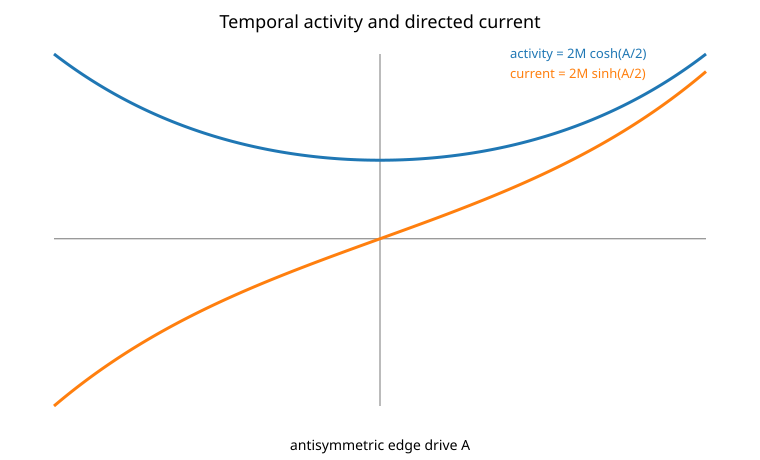
\includegraphics[width=0.86\textwidth]{figures/temporal_activity_decomposition.png}
\caption{Reference decomposition of one directed kinetic pair at fixed mobility $M=1$. Positive activity is even in the edge drive, while directed current is odd. The figure is generated by \texttt{scripts/build\_temporal\_activity\_figure.py}.}
\label{fig:temporal-activity-decomposition}
\end{figure}

\chapter{Causal Bifurcation}
At a localized transition event,
\[
\Psi_T(s_n^+)=B(q_n)\Psi_T(s_n^-).
\]
The next derivation must classify admissible bifurcation operators by identity limit, composition law, invertibility and information change.

\chapter{Temporal Transport and Internal Elapsed Activity}

Temporal Transport composes smooth Temporal Wave evolution with the localized bifurcation events supplied by the wave-active NOW carrier.

\section{Smooth Temporal Wave segment}

Let
\[
K=K_M\succeq0,
\qquad
C=C_\eta\succeq0,
\]
and use the phase-space state
\[
x=\begin{pmatrix}q\\p\end{pmatrix}.
\]
The smooth generator is
\[
\boxed{
A_W=
\begin{pmatrix}
0&-I\\
K&-C
\end{pmatrix}.
}
\]
The wave energy has metric
\[
\boxed{
Q_W=
\begin{pmatrix}
K&0\\
0&I
\end{pmatrix},
}
\]
with
\[
\mathcal H_T=\frac12x^\dagger Q_Wx.
\]
A direct calculation gives
\[
\boxed{
A_W^\dagger Q_W+Q_WA_W
=
\begin{pmatrix}
0&0\\
0&-2C
\end{pmatrix}\preceq0.
}
\]

For an ordered increment $h>0$, the reference smooth segment is the Cayley transform
\[
\boxed{
U_h^{(W)}
=\left(I-\frac h2A_W\right)^{-1}
\left(I+\frac h2A_W\right).
}
\]
It obeys the exact discrete energy inequality
\[
\boxed{
(U_h^{(W)})^\dagger Q_WU_h^{(W)}\preceq Q_W.
}
\]
For $C=0$ the inequality becomes equality, giving a $Q_W$-unitary conservative segment.

\section{Interrupted transport}

For smooth segments $U_n$ and localized event operators $B_n$, chronological transport is
\[
\boxed{
\mathcal U_{f\leftarrow i}
=U_NB_NU_{N-1}B_{N-1}\cdots U_1B_1U_0.
}
\]
The multiplication order is inherited from the ordered event sequence.

A sufficient energy-compatible event condition is
\[
[G_n,Q_W]=0
\]
for the Hermitian directional generator $G_n$.  Then
\[
B_n=e^{-i\beta_nG_n}
\]
satisfies
\[
B_n^\dagger Q_WB_n=Q_W.
\]
For one shared wave-energy metric, a product of $Q_W$-contractive smooth segments and $Q_W$-unitary realized events obeys
\[
\boxed{
\mathcal U_{f\leftarrow i}^\dagger
Q_W
\mathcal U_{f\leftarrow i}
\preceq Q_W.
}
\]
The generic interrupted-product contract also retains its spectral-norm bound, exact cut identity and conditioning audit.

\section{Internal elapsed activity}

The positive activity layer defines an internal elapsed coordinate before metric-clock calibration. Let $\lambda$ be an admissible increasing ordering parameter, let $\mathfrak a(\lambda)>0$ denote realized temporal activity, and let $\mathfrak a_\star>0$ be a declared system-internal reference activity. Define
\[
\boxed{
d\tau_{\rm int}
=\frac{\mathfrak a(\lambda)}{\mathfrak a_\star}\,d\lambda.
}
\]
For a discrete ordered path,
\[
\boxed{
\tau_{{\rm int},N}
=\sum_{n=0}^{N-1}
\frac{\mathfrak a_n}{\mathfrak a_\star}\,\Delta\lambda_n,
\qquad
\Delta\lambda_n>0.
}
\]
Every admitted increment is strictly positive, so the internal elapsed coordinate is strictly monotone along the realized ordered path.

\section{Reparameterization covariance}

For an increasing relabeling $\lambda'=f(\lambda)$, let activity transform as a one-density,
\[
\mathfrak a'(\lambda')
=\mathfrak a(\lambda)\frac{d\lambda}{d\lambda'}.
\]
Then
\[
\mathfrak a'(\lambda')\,d\lambda'
=\mathfrak a(\lambda)\,d\lambda,
\]
and hence
\[
\boxed{d\tau'_{\rm int}=d\tau_{\rm int}.}
\]

\section{Relational density, viscosity and internal pace}

Using
\[
\mathfrak a_{ab}
=2M_{ab}\cosh(A_{ab}/2),
\]
with
\[
M_{ab}
=\frac{\sqrt{\rho_R(a)\rho_R(b)}}{\tfrac12[\eta_R(a)+\eta_R(b)]},
\]
gives
\[
\boxed{
\frac{d\tau_{\rm int}}{d\lambda}
=\frac{2}{\mathfrak a_\star}
\frac{\sqrt{\rho_R(a)\rho_R(b)}}{\tfrac12[\eta_R(a)+\eta_R(b)]}
\cosh(A_{ab}/2).
}
\]
Within this candidate, relational density raises the internal activity pace and relational viscosity lowers it. Reversing the antisymmetric drive leaves the pace invariant while the directed current reverses sign.

The resulting transport layer therefore carries both an ordered state propagator and the system-internal elapsed-activity coordinate consumed by the Memory node.

\chapter{Memory and Retrodiction}

The memory layer is developed downstream of Temporal Transport. The current executable branch combines the existing oriented memory coordinate with a Kepler--Newton evolution law parameterized by the internal elapsed activity variable.

\section{Oriented memory coordinate}

Assign a complex memory coordinate
\[
m(s)=x_M(s)+iy_M(s)=r_M(s)e^{i\theta_M(s)}.
\]
The oriented edge functional is
\[
\boxed{
A^{(M)}_{ab}
=\lambda_M\operatorname{Im}[m(a)^*m(b)]
=\lambda_M r_a r_b\sin(\theta_b-\theta_a).
}
\]
For a closed polygonal orbit,
\[
\sum_C A^{(M)}_e
=2\lambda_M\mathcal A_M(C),
\]
where \(\mathcal A_M(C)\) is the signed enclosed area.

\section{Internal-time Newton dynamics}

The internal evolution increment inherited from temporal activity is
\[
d\tau_{\rm int}=\frac{\mathfrak a}{\mathfrak a_\star}\,d\lambda.
\]
On the memory plane we introduce the effective central parameter \(\mu_M>0\) and
\[
V_M(r_M)=-\frac{\mu_M}{r_M}.
\]
The smooth memory trajectory obeys
\[
\boxed{
\frac{d^2m}{d\tau_{\rm int}^2}
=-\mu_M\frac{m}{|m|^3}.
}
\]
The origin and calibration of \(\mu_M\) remain an explicit derivation target.

\section{Kepler structure}

Define
\[
\varepsilon_M
=\frac12\left|\frac{dm}{d\tau_{\rm int}}\right|^2
-\frac{\mu_M}{r_M},
\qquad
h_M
=\operatorname{Im}\!\left[m^*\frac{dm}{d\tau_{\rm int}}\right].
\]
The central-force law gives the areal relation
\[
\boxed{
\frac{d\mathcal A_M}{d\tau_{\rm int}}
=\frac{h_M}{2}.
}
\]
The corresponding conic is
\[
r_M(\nu)
=\frac{p_M}{1+e_M\cos\nu},
\qquad
p_M=\frac{h_M^2}{\mu_M}.
\]
For a bound nondegenerate orbit,
\[
a_M=-\frac{\mu_M}{2\varepsilon_M},
\qquad
T_M^2=\frac{4\pi^2}{\mu_M}a_M^3.
\]
Combining the areal law with the earlier memory circulation yields
\[
\boxed{
\frac{d}{d\tau_{\rm int}}
\left(\sum_C A_e^{(M)}\right)
=\lambda_M h_M.
}
\]

\section{Bifurcation impulse}

A localized event can modify the orbital state through
\[
\boxed{
\mathbf v_M^+
=\mathbf v_M^-+\Delta\mathbf v_M.
}
\]
The event-imprint projection that generates \(\Delta\mathbf v_M\) is kept as a separate derivation target. The resulting orbital state can be classified by \(\varepsilon_M\), \(h_M\), eccentricity and the conic branch.

The current numerical reference uses velocity--Verlet propagation and records targeted structural tests in \texttt{validation/KEPLER\_MEMORY\_DYNAMICS\_V0\_1.json}. Retrodiction opens after the memory update law receives its own admission receipt.

\chapter{Memory Integration Gate}

The Memory node is assembled from components derived and validated in the preceding layers. The structural reference path used by the current integration gate is
\[
\boxed{
\mathbb{CP}^1\ \text{state geometry}
\longrightarrow
\delta m_n
\longrightarrow
q_n\delta m_n
\longrightarrow
\mathcal C_n
\longrightarrow
\mathcal E_n
\longrightarrow
\operatorname{RECALL}.
}
\]

For the \(\mathbb{CP}^1\) K\"ahler-frame reference subclass,
\[
|\delta m_n|=d_{FS}(a,b).
\]
Together with the upstream-derived event kick,
\[
\Delta v_{M,n}=q_n\delta m_n,
\]
this gives the integrated magnitude identity
\[
\boxed{
|\Delta v_{M,n}|=q_n d_{FS}(a,b).
}
\]
The subsequent memory lineage cell is
\[
\mathcal C_n
=\Phi_K(\Delta\tau_n;\mu_M)\circ K_{\mathcal E_n},
\qquad
\mathcal E_n=(\Delta\tau_n,q_n,\delta m_n).
\]
The append-only ledger therefore carries the quantities required by the declared inverse reference cell and ledger-assisted reconstruction.

\section{Integrated controls}

The dedicated integration test composes two non-collinear CP1 events with event weighting, Kepler propagation and recall. The targeted reference checks verify Fubini--Study normalization, event-kick scaling, complete multi-event reconstruction, recovery of intermediate checkpoints, upstream global-phase invariance and a tampered-receipt negative control. A zero-weight event also preserves reversible smooth propagation.

These controls are recorded in
\texttt{validation/MEMORY\_ADMISSION\_V0\_1.json}.
The isolated integration harness passed all six test functions represented by
\texttt{tests/reference/test\_memory\_admission.py}.

\section{Temporal Transport parent bridge}

The smooth Temporal Transport segment already carries an ordered increment \(\Delta\lambda_n>0\). Together with the positive transition activity it supplies the Memory duration
\[
\boxed{
\Delta\tau_n
=\frac{\mathfrak a_n}{\mathfrak a_\star}\Delta\lambda_n.
}
\]
The declared one-density transformation of \(\mathfrak a\) makes this increment invariant under increasing reparameterization of \(\lambda\).

The wave-active NOW layer supplies the non-negative realization weight
\[
r_n^{(W)}=q_n\epsilon_n^{(W)}
\]
and the exact support gate
\[
g_n=\mathbf 1[r_n^{(W)}>0].
\]
The transport-derived Memory receipt is therefore
\[
\boxed{
\mathcal E_n^{T\to M}
=(\Delta\tau_n,g_nq_n,\delta m_n).
}
\]
Thus Temporal Wave activation controls whether the localized transition writes a kick, while the already derived structural event signature remains the normalized kick amplitude:
\[
\boxed{
\Delta v_{M,n}=g_nq_n\delta m_n.
}
\]
A wave-inactive event has zero kick and still advances the smooth Memory segment through its positive \(\Delta\tau_n\).

The product \(q_n\epsilon_n^{(W)}\) remains a NOW realization/provenance weight. The admitted Memory kick continues to use \(g_nq_n\delta m_n\), because \(\epsilon_n^{(W)}\) rescales as \(|c|^2\) under \(\Phi\mapsto c\Phi\), whereas its positive support is invariant for \(c\neq0\). Identification of the wave-amplitude factor with a kick amplitude therefore belongs to a separate upstream normalization gate.

A deterministic 5,000-case bridge probe returned zero support-gate failures, reparameterization defect below \(1.8\times10^{-15}\), and forward/reverse lineage reconstruction defect below \(4.9\times10^{-13}\). GREMLIN evaluated the bridge in \texttt{CANDIDATE\_ONLY} mode and all three declared hypotheses returned \texttt{SUPPORTED\_BY\_DECLARED\_TESTS}.

\section{Hosted full reference suite}

The previously outstanding repository-wide gate was executed on 28 August 2026 by the GitHub Actions \texttt{Reference suite} workflow. The exact PR merge of source commit
\texttt{3ac1f53af5223d16f8818dba99a63a6af2ba9498}
with the evidence-only branch was tested under Python 3.12.14 on Ubuntu 24.04 using
\begin{verbatim}
python -m pytest -q tests/reference
\end{verbatim}
The suite completed with
\begin{verbatim}
431 passed in 7.08s
\end{verbatim}
and the workflow, job, and test step all concluded successfully. The tested merge commit is
\texttt{e0b1cdc491a1a501adce93b8d62ade063e167500}
with tree
\texttt{92302498f3c9131b163d5d0ccbbeab1db935d29f}.

The append-only evidence binding is recorded in
\texttt{validation/MEMORY\_ADMISSION\_HOSTED\_FULL\_SUITE\_2026\_08\_28.json}.

This closes the declared full-suite blocker for the integrated Memory reference gate. The proposed post-merge status at this recorded checkpoint is therefore
\[
\boxed{\mathrm{Memory}:\ \mathrm{REFERENCE\ GATE\ ADMITTED}.}
\]
At this checkpoint ORCHORBITAL was the next separate dependency gate. The later ORCHORBITAL chapters record its residence/switch provenance, hierarchical attractor families, typed-observable admission and hosted admission receipt before Retrodiction advances downstream.

\chapter{Retrodiction as a Withheld-Lineage Inverse Problem}

This chapter records a provisional downstream Retrodiction reference candidate. The canonical dependency frontier remains at Memory until the integrated Memory tree obtains its full repository reference-suite admission result. The purpose of this chapter is therefore to define the inverse problem without advancing the admitted frontier.

\section{Recall versus retrodiction}

For a complete persisted event ledger, recall applies the known inverse cells
\[
\operatorname{RECALL}_{N\to0}
=\mathcal C_0^{-1}\mathcal C_1^{-1}\cdots\mathcal C_{N-1}^{-1}.
\]
Retrodiction begins when part of the lineage is withheld and must be inferred from the remaining constraints.

Consider one memory cell
\[
X_{n+1}
=\Phi_K(\Delta\tau_n;\mu_M)
\circ K(q_n,\delta m_n)
\,X_n,
\]
where
\[
K(q_n,\delta m_n):
\quad v_M\mapsto v_M+q_n\delta m_n.
\]
The reference problem retains the checkpoints \(X_n\) and \(X_{n+1}\), the smooth-step duration \(\Delta\tau_n\) and \(\mu_M\), while withholding one factor of the event receipt.

\section{Missing-kick reconstruction}

Reverse only the known smooth Kepler segment:
\[
\widetilde X_n
=\Phi_K^{-1}(\Delta\tau_n;\mu_M)X_{n+1}.
\]
The reconstructed kick is
\[
\boxed{
\Delta v_{M,n}
=\widetilde v_{M,n}-v_{M,n}.
}
\]
The reference implementation requires the recovered position, internal elapsed activity and swept area to agree with the retained pre-event checkpoint within the declared tolerance. A checkpoint mismatch fails closed.

\section{Conditional identifiability of the event weight}

If a nonzero memory imprint \(\delta m_n\) is independently supplied by the upstream state-geometry layer, then
\[
\boxed{
\widehat q_n
=
\frac{\operatorname{Re}(\Delta v_{M,n}\delta m_n^*)}
{|\delta m_n|^2}.
}
\]
The factorization residual is
\[
\boxed{
r_n
=\Delta v_{M,n}-\widehat q_n\delta m_n.
}
\]
The reference contract requires \(\widehat q_n\ge0\) and a residual below the declared tolerance. Thus a wrong imprint direction is rejected rather than silently absorbed into the scalar estimate.

For the \(\mathbb{CP}^1\) memory-frame reference subclass, the upstream normalization
\[
|\delta m_n|=d_{FS}
\]
provides an independently defined imprint scale.

\section{Conditional identifiability of the memory imprint}

If \(q_n>0\) is independently known while the imprint is withheld, then
\[
\boxed{
\widehat{\delta m}_n
=\frac{\Delta v_{M,n}}{q_n}.
}
\]
For \(q_n=0\), consistency requires a zero kick in the reference cell.

\section{Product-only ambiguity}

If both factors are withheld, the checkpoints determine only the product. For every positive scalar \(c\),
\[
\boxed{
(q_n,\delta m_n)
\mapsto
(cq_n,\delta m_n/c)
}
\]
leaves
\[
q_n\delta m_n
\]
unchanged. Therefore the factorization is non-identifiable from the memory checkpoints alone. The implementation reports this ambiguity explicitly and does not choose an arbitrary decomposition.

\section{Multi-event observability before estimation}

For \(N\) latent event kicks, collect
\[
z=(u_1,\ldots,u_N)\in\mathbb R^{2N},
\]
where each \(u_k\) is the two-component memory-velocity jump. Retained post-event checkpoints define a measurement map \(Y(z)\). At a nominal lineage \(z_0\), define
\[
\boxed{
J_R(z_0)=\left.\frac{\partial Y}{\partial z}\right|_{z_0}.
}
\]
The first-order local-identifiability gate is
\[
\boxed{\operatorname{rank}J_R=2N.}
\]
The singular spectrum is retained separately to distinguish full rank from poor conditioning.

One final memory phase-state checkpoint carries four real coordinates,
\[
Y_f=(r_x,r_y,v_x,v_y)\in\mathbb R^4,
\]
so
\[
J_R^{\rm final}\in\mathbb R^{4\times2N},
\qquad
\boxed{\operatorname{rank}J_R^{\rm final}\le4.}
\]
Consequently,
\[
\boxed{
N>2
\Longrightarrow
4<2N
\Longrightarrow
\text{final-only reconstruction is dimensionally underdetermined}.
}
\]
This obstruction is established before fitting or optimization.

If a checkpoint set \(\mathcal C\) is retained, then
\[
Y_{\mathcal C}\in\mathbb R^{4|\mathcal C|},
\]
and a necessary dimensional condition becomes
\[
\boxed{4|\mathcal C|\ge2N.}
\]
The actual full-column-rank condition must still be checked. In the targeted three-kick reference case, one final checkpoint gives a \(4\times6\) underdetermined matrix, whereas retaining all three post-event checkpoints gives a \(12\times6\) sensitivity matrix with rank six.

\section{Gated latent-lineage estimation}

Once the observability gate passes, the provisional reference estimator solves
\[
\boxed{
\widehat z
=\arg\min_z\frac12\|Y_{\rm obs}-Y(z)\|_2^2.
}
\]
Writing
\[
r_k=Y_{\rm obs}-Y(z_k),
\qquad
J_k=J_R(z_k),
\]
the damped Gauss--Newton proposal is defined by
\[
\boxed{
(J_k^T J_k+\lambda I)\delta z_k
=J_k^T r_k,
\qquad \lambda\ge0.
}
\]
The reference line search accepts only \(\alpha=2^{-j}\) satisfying
\[
\|Y_{\rm obs}-Y(z_k+\alpha\delta z_k)\|_2
<\|r_k\|_2.
\]
Loss of full column rank, singular normal equations or absence of an admitted descent step terminates the reference estimate explicitly.

\section{Estimate commitment and reference nulls}

The estimator interface contains the retained observations and public forward-model quantities. The estimate is frozen before sealed truth enters scoring through
\[
\boxed{
C_{\rm est}
=\operatorname{SHA256}(\widehat z\,\|\,\widehat Y\,\|\,r\,\|\,\mathrm{metadata}).
}
\]
The scorer verifies this commitment before reconstruction error is evaluated.

Two dynamical reference nulls are carried with the same experiment. The zero-kick null fixes
\[
z=0
\]
and records residual \(r_0\). The checkpoint-order null reverses the complete four-component checkpoint blocks and applies the same estimator capacity, giving fitted residual \(r_{\rm shuf}\). Their reference reductions are
\[
\boxed{
R_0=1-\frac{r_{\rm est}}{r_0},
\qquad
R_{\rm shuf}=1-\frac{r_{\rm est}}{r_{\rm shuf}}.
}
\]
Their registered evidence class is \texttt{COMPUTATIONAL\_REFERENCE\_DIAGNOSTIC}; physical significance evaluation remains a later evidence gate.

In the first exact three-event reference run, the \(12\times6\) observability matrix has rank six. The estimator converges in two iterations with residual approximately \(1.04\times10^{-14}\). The zero-kick residual is approximately \(9.20\times10^{-2}\), while the reversed-checkpoint fit stalls at approximately \(9.57\times10^{-2}\). Fifty seeded exact-reference cases all retain full rank and converge, with maximum recorded kick-coordinate error approximately \(1.65\times10^{-14}\).

\section{Reference controls and evidence boundary}

Single-missing-receipt controls are recorded in
\texttt{validation/RETRODICTION\_SINGLE\_MISSING\_RECEIPT\_V0\_1.json},
the multi-event rank audit in
\texttt{validation/RETRODICTION\_OBSERVABILITY\_V0\_1.json},
and the gated estimator/null controls in
\texttt{validation/RETRODICTION\_ESTIMATION\_NULLS\_V0\_1.json}.
The isolated reference harnesses cover missing-kick reconstruction, conditional factor identification, product-only ambiguity, collinearity rejection, checkpoint tampering, dimensional underdetermination, checkpoint-augmented rank recovery, gated multi-kick estimation, estimate commitment and the declared reference nulls. The observability layer reports `UNDERDETERMINED_DIMENSION`, `RANK_DEFICIENT`, or `LOCALLY_IDENTIFIABLE_REFERENCE` according to the measured sensitivity structure.

This evidence belongs to a provisional downstream formal reference class. Retrodiction admission remains gated by the parent Memory admission result. Retrocausal tests remain a later dependency node with their own statistical, leakage and classical-channel audits.

\chapter{Retrocausality}
Status: deferred until its dependency frontier is admitted.

\chapter{Experiments and Falsification}

\noindent\textbf{Status:} \texttt{REFERENCE-MODEL TESTS ACTIVE / PHYSICAL TESTS PREREGISTERED / EVIDENCE-CLASS SEPARATION REQUIRED}.

The experimental programme of Informational Dynamics of Time is organised as a sequence of increasingly demanding tests. The purpose of the sequence is to preserve a strict distinction between an algebraic identity, a deterministic reference-model reconstruction, a statistical anomaly, and a measured physical result. The temporal formalism therefore reaches experiment through explicit interfaces rather than through a single omnibus claim.

The canonical progression is
\[
\boxed{
\text{formal identity}
\longrightarrow
\text{reference implementation}
\longrightarrow
\text{withheld-variable test}
\longrightarrow
\text{preregistered physical test}
\longrightarrow
\text{independent replication}
}.
\]
Each promotion requires its own evidence receipt.

\section{Experimental observables of the temporal branch}

The temporal primitive supplies a positive activity measure
\[
d\Theta=\mathfrak a\,d\lambda,
\qquad \mathfrak a>0,
\]
and the local/reference comparison supplies the relational lapse
\[
N_R(x|r)=\frac{d\Theta_x}{d\Theta_r}
=\frac{\mathfrak a_x}{\mathfrak a_r}>0.
\]
Once a reference clock is physically calibrated by
\[
dt=T_r\,d\Theta_r,
\]
the local calibrated elapsed interval is
\[
d\widehat\tau_x=N_R(x|r)\,dt.
\]
This identifies the first experimental class: measurements of relative clock rate under independently characterised relational conditions. The primary observable is a dimensionless clock ratio, while conversion to seconds belongs to the calibration layer.

A second class concerns phase transport. On an admitted physical-clock calibration domain, the temporal branch is tested against the phase relation
\[
\Delta\phi_t=-\frac{E\Delta t}{\hbar}.
\]
The associated failure coordinate is direct: the temporal transport construction must recover the physical phase relation from its admitted bridge assumptions rather than by redefining the measured phase after the fact.

A third class concerns memory and retrodiction. Here the observable data are ordered checkpoints, event receipts, residence cells, winding increments, radial coordinates, and final retained states. These tests are especially useful because they permit exact withheld-lineage experiments before any physical retrocausal interpretation is considered.

\section{E003: withheld-lineage retrodiction}

The E003 protocol tests whether deliberately hidden lineage variables can be reconstructed from permitted checkpoints and declared model parameters. Its reference dynamics are
\[
X_{k+1}
=
\Phi_K(\Delta\tau_k;\mu_M)
\circ K_{u_k}(X_k),
\qquad
u_k=q_k\,\delta m_k,
\]
where the smooth Kepler-memory segment and the event kick are independently typed operations. The sealed truth variables are excluded from the estimator input.

The protocol contains several distinct identifiability regimes. If one factor of the event product is independently known, the complementary factor can be reconstructed from the inferred kick. If both \(q_k\) and \(\delta m_k\) are hidden, the event product remains the identifiable coordinate and factorisation is treated as a separate ambiguity class. Multi-event reconstruction is audited through the observation Jacobian
\[
J_R=\frac{\partial Y_C}{\partial z}.
\]
For a latent coordinate of dimension \(2N\), local observability requires
\[
\operatorname{rank}J_R=2N.
\]
A final-only multi-kick configuration supplies a mandatory underdetermined control.

The covariance-weighted residual is
\[
Q(z)=r(z)^T\Sigma_Y^{-1}r(z),
\]
and chronology controls are generated by checkpoint-block permutations with the same nominal information capacity. This separates reconstruction driven by ordered lineage from reconstruction achievable after chronology is destroyed.

The first reference run used three kicks, a six-dimensional latent coordinate, and a twelve-dimensional observation coordinate. The observability rank was six. The estimator converged in two iterations, with residual of order \(10^{-14}\) and maximum kick error of order \(10^{-14}\). Fifty randomised reference cases retained full rank and converged within the same numerical scale. The zero-kick and shuffled-chronology controls produced residuals many orders of magnitude larger than the exact reference solution.

The weighted diagnostic run again obtained rank six, with a modest condition number, while all tested nonidentity chronology permutations generated very large weighted residuals. The permutation ensemble in this diagnostic is an observability stress test rather than a sampling-based physical significance calculation.

The experimental meaning of E003 is therefore precise. It establishes that the admitted memory dynamics and observation map support exact reconstruction in the declared reference class, with controls for hidden-truth leakage, product ambiguity, rank deficiency, and chronology destruction. Its evidence class is \texttt{PASS\_MODEL\_INTERNAL} when the stated gates pass.

\section{Residence-bound compressed reconstruction}

The retrodiction carrier has been reduced from a full Cartesian packet to a winding--radius packet on each admitted active-attractor stratum. With
\[
\rho_k=\|r_k-c_{a_k}\|>0,
\]
and ordered winding increments \(\Delta W_k\), the pre-final positions are reconstructed by
\[
r_k=c_{a_k}+\rho_k
\begin{pmatrix}
\cos(\theta_{k-1}^{(a_k)}+2\pi\Delta W_k)\\
\sin(\theta_{k-1}^{(a_k)}+2\pi\Delta W_k)
\end{pmatrix}.
\]
The radial packet contains \(N-1\) new scalar coordinates in place of the \(2N-2\) Cartesian coordinates of the baseline carrier. Thus
\[
\boxed{
\frac{N_{\rm radial}}{N_{\rm Cartesian}}=\frac12
}
\]
for \(N>1\).

The 07V residence binding attaches every retained radius to the checkpoint index, active attractor, exact binary64 radius, source residence cell, post-segment state commitment, and preceding radial commitment. The content-addressed chain therefore supplies provenance for the compressed coordinate used by the decoder. The hosted reference suite for this gate passed 557 tests. The broader global injectivity coordinate remains a separate frontier beyond the declared positive-radius stratified domain.

\section{E004: prospective retrocausal discrimination}

Chapter~9 defines the preregistration boundary for a genuinely retrocausal candidate. The primary statistical target is
\[
P(X_{\mathrm{past}}\mid Y_{\mathrm{future}})
\stackrel{?}{\neq}
P(X_{\mathrm{past}}),
\]
with the future condition selected after the earlier measurement event and with the complete analysis contract committed beforehand.

Admission of a physical candidate requires, at minimum, cryptographic timestamp commitments, blinded future-condition assignment, a classical-channel audit, shared-clock and scheduler controls, sham/null trials, a fixed exclusion policy, and replication. The raw earlier record is immutable. Analysis proceeds from committed data products and an analysis plan whose hash predates condition unblinding.

The result ladder used throughout this programme is
\[
\texttt{RAW\_OBSERVATION}
\rightarrow
\texttt{STATISTICAL\_EFFECT}
\rightarrow
\texttt{CLASSICAL\_CHANNEL\_AUDIT}
\rightarrow
\texttt{PHYSICAL\_CLAIM\_STATUS}.
\]
A statistical deviation is therefore only one coordinate of the experimental conclusion.

\section{Falsification matrix}

The experimental programme contains five principal falsification families.

\begin{enumerate}
\item \textbf{Temporal phase transport.} Test recovery of \(\Delta\phi_t=-E\Delta t/\hbar\) on the declared calibration domain.
\item \textbf{Spacetime closure.} Combine the independently developed temporal and spatial branches and test the reconstructed phase against
\[
\Delta\phi=\frac{1}{\hbar}
\left(\mathbf p\cdot\Delta\mathbf x-E\Delta t\right).
\]
\item \textbf{NOW and bifurcation.} Test branch integrity, realised-lineage uniqueness, reconstructive reversibility where specified, and repeated-state re-entry consistency.
\item \textbf{Retrodiction and retrocausal discrimination.} Use E003 for model-internal reconstruction and E004 for the preregistered physical candidate test.
\item \textbf{Bell/CHSH discrimination where the experimental topology requires it.} For independently selected settings \(a,a',b,b'\), evaluate
\[
S=E(a,b)+E(a,b')+E(a',b)-E(a',b'),
\]
with explicit timing, selection, detection, and communication controls.
\end{enumerate}

\section{Evidence classes and provenance}

The canonical verdict classes are
\[
\begin{gathered}
\texttt{PASS\_MODEL\_INTERNAL},\quad
\texttt{FAIL\_MODEL\_INTERNAL},\quad
\texttt{CLASSICAL\_COMPATIBLE},\\
\texttt{ANOMALY\_CANDIDATE},\quad
\texttt{RETROCAUSAL\_CANDIDATE},\quad
\texttt{NONCLASSICAL\_CORRELATION\_CANDIDATE},\\
\texttt{MEASURED\_PHYSICAL\_RESULT}.
\end{gathered}
\]
Every promoted result retains the raw-data identity, source commit, parameter manifest, test coordinate, uncertainty model, and failure receipt. This provenance rule is part of the scientific content of the programme: a temporal claim is evaluated together with the chronology by which its evidence was produced.

The resulting experimental architecture mirrors the theory itself. Temporal order generates an observable lineage; memory makes that lineage addressable; retrodiction tests whether the retained structure is sufficient to reconstruct hidden causes; preregistration then supplies the boundary at which a future-conditioned physical effect can be distinguished from reconstruction, leakage, scheduling, and ordinary forward causation.

\chapter{Space as an External Branch}
Status: deferred until its dependency frontier is admitted.

\chapter{Einstein Interface and Closure Tests}

\noindent\textbf{Status:} \texttt{STANDARD GR IDENTITIES RECOVERED / IDT-TO-GR BINDING CONDITIONAL / CONSERVATION GATES EXPLICIT / CROSS-SYSTEM UNIVERSALITY ACTIVE}.

This chapter is a downstream interface chapter. It does \emph{not} claim to derive general relativity, the Einstein tensor, the Einstein coupling, Maxwell theory, or Hawking thermodynamics from the IDT primitives. Those are established physical structures used here as recovery benchmarks and closure constraints. The IDT-specific question is narrower and testable: whether the independently constructed temporal outputs and source interfaces can be bound to those structures without circularly defining the quantities that are later used for confirmation.

\section{Standard geometric benchmark}

For a metric-compatible spacetime connection, define
\[
G_{\mu\nu}=R_{\mu\nu}-\frac12Rg_{\mu\nu}.
\]
The contracted Bianchi identity gives
\[
\boxed{\nabla^\mu G_{\mu\nu}=0.}
\]
Together with the standard Einstein field equation \cite{Einstein1916},
\[
\boxed{
G_{\mu\nu}+\Lambda g_{\mu\nu}
=
\kappa_E T^{\rm total}_{\mu\nu},
\qquad
\kappa_E=\frac{8\pi G}{c^4},
}
\]
this requires a conserved total source on the admitted equations. The value of \(\kappa_E\) is imported from standard gravitational physics; it is not newly derived by the present temporal formalism.

The conservation role of continuous symmetries belongs to the standard Noether framework \cite{Noether1971}. In this monograph, the novelty test is therefore not whether the Bianchi identity or Noether theorem holds, but whether the IDT source and temporal interfaces enter a conservation-compatible ledger without hidden source terms or post-hoc normalization.

\section{Electromagnetic source bridge}

The phase connection can be compared with the standard Aharonov--Bohm phase normalization \cite{AharonovBohm1959},
\[
a_{AB}=\frac{q}{\hbar}A,
\qquad
F=dA.
\]
The repository-level source convention binds
\[
\boxed{
J_{\rm EM}^{\mu}=\frac{1}{\hbar}\,\mathcal J_Q^{\mu},
}
\]
and, for a single carrier satisfying the declared identification gate,
\[
J_{\rm EM}^{\mu}=\frac{q}{\hbar}J_{\vartheta}^{\mu}.
\]

The standard electromagnetic stress tensor is
\[
\boxed{
T^{\rm EM}_{\mu\nu}
=
\frac{1}{\mu_*}
\left(
F_{\mu\alpha}F_{\nu}{}^{\alpha}
-\frac14g_{\mu\nu}F_{\alpha\beta}F^{\alpha\beta}
\right).
}
\]
The unit ledger takes \(\mu_*=1\) in Heaviside--Lorentz natural units and \(\mu_*=\mu_0\) in SI. These equations serve as a recovery and normalization benchmark for the source adapter, not as a new electromagnetic derivation.

\section{Matter exchange and total conservation}

On the admitted Maxwell--matter equations,
\[
\nabla^\mu T^{\rm EM}_{\mu\nu}
=-F_{\nu\lambda}J_{\rm EM}^{\lambda},
\qquad
\nabla^\mu T^{\rm matter}_{\mu\nu}
=+F_{\nu\lambda}J_{\rm EM}^{\lambda},
\]
so that
\[
\boxed{
T^{\rm total}_{\mu\nu}
=T^{\rm EM}_{\mu\nu}+T^{\rm matter}_{\mu\nu}
}
\]
obeys
\[
\boxed{\nabla^\mu T^{\rm total}_{\mu\nu}=0.}
\]
This is the conservation gate required by the standard geometric side. The IDT closure task is to show that every promoted additional source contributes to the same ledger and that no source is silently omitted.

\section{Temporal lapse as the independent IDT input}

The temporal branch exports
\[
\Theta_R=N_Rc\,dt,
\qquad
N_R=\frac{\mathfrak a_x}{\mathfrak a_r}>0.
\]
Together with an independently admitted spatial triad \(e^{\hat i}\), this gives the candidate spacetime coframe
\[
\mathcal E=(\Theta_R,e^{\hat1},e^{\hat2},e^{\hat3}).
\]
The weak temporal scalar
\[
\Phi_N=c^2\ln N_R
\]
is a comparison coordinate for clock-redshift tests.

The physically discriminating closure condition is not the algebraic equality obtained by defining one side from the other. It is the held-out comparison
\[
\boxed{
\widehat N_R^{\,\rm IDT}(x|r)
\stackrel{\rm test}{=}
N_R^{\rm geometric}(x|r),
}
\]
where \(\widehat N_R^{\,\rm IDT}\) must be computed from independently measured or preregistered relational observables and frozen parameters that exclude the target clock ratio. If the observed clock ratio, the geometric lapse, or a fitted equivalent is used to define \(\mathfrak a_x/\mathfrak a_r\), the result is a calibration or consistency check rather than an independent prediction.

\section{Dynamic vacuum bookkeeping}

A spacetime-dependent scalar vacuum term may be written as \(\Lambda_0(x)\). If
\[
G_{\mu\nu}+\Lambda_0g_{\mu\nu}
=
\kappa_E T^{\rm total}_{\mu\nu},
\]
then Bianchi compatibility requires
\[
\boxed{
\kappa_E\nabla^\mu T^{\rm total}_{\mu\nu}
=
\nabla_\nu\Lambda_0.
}
\]
Equivalently,
\[
T^\Lambda_{\mu\nu}
=-\frac{\Lambda_0}{\kappa_E}g_{\mu\nu}
\]
must be included in the total conserved bookkeeping. This is a consistency condition only. A first-principles dynamical action and independently testable source model for any promoted \(\Lambda_0(x)\) remain open.

\section{Directional-stress recovery channel}

For an admitted ultrarelativistic directional source,
\[
T_\nu^{\mu\nu}
=
\sum_a u_a k_a^\mu k_a^\nu.
\]
The transverse-traceless components
\[
T_+=\frac12(T_{xx}-T_{yy}),
\qquad
T_\times=T_{xy},
\]
and the linearized far-zone relation
\[
\boxed{
h_{ij}^{TT}
=
\frac{4G}{c^4r}\,\mathcal T_{ij}^{TT}
}
\]
belong to the standard linearized-gravity benchmark. The IDT programme contributes a proposed source adapter and provenance/calibration contract. A physical result requires response-corrected data, uncertainty propagation, and a source model frozen independently of the measured gravitational response. Isotropic directional ensembles provide a built-in null.

\section{Horizon recovery benchmark}

The Euclidean non-extremal horizon relations
\[
\beta_H=\frac{2\pi}{\kappa_H},
\qquad
\oint\kappa_Hd\tau_E=2\pi,
\]
and
\[
\boxed{
T_H=\frac{\hbar\kappa_H}{2\pi c k_B}
}
\]
are standard black-hole thermodynamic results associated with Hawking radiation and Euclidean regularity \cite{Hawking1975,GibbonsHawking1977}. Likewise, the periodic/antiperiodic thermal boundary conditions for integer- and half-integer-spin fields are recovery constraints on any compatible microscopic model. Reproducing these relations is scientifically necessary but is not, by itself, a novel prediction of IDT.

\section{Closure verdict semantics}

The present chapter establishes a typed \emph{interface}, not a completed empirical derivation of gravity from information. A successful closure claim requires all of the following:
\begin{enumerate}
\item the temporal predictor is generated independently of the target clock/geometric measurement;
\item every promoted source is included in a conservation-compatible stress ledger;
\item standard GR and field-theory limits are recovered without parameter definitions that encode the target result;
\item at least one held-out observable can distinguish the IDT bridge from the declared baseline;
\item the result survives uncertainty propagation and, for a physical promotion, independent replication.
\end{enumerate}

The current mathematical result is therefore a conservation-compatible path from declared temporal/source variables to the Einstein--Bianchi interface. The remaining physical question is whether nature realizes that path with independently measurable IDT variables.

\chapter{Predictions, Recovery Benchmarks, and Discriminators}

\noindent\textbf{Status:} \texttt{MODEL-INTERNAL CONSEQUENCES / STANDARD-PHYSICS RECOVERY / DISCRIMINATING TESTS EXPLICITLY SEPARATED}.

This chapter uses the word \emph{prediction} only for a quantity that is fixed before the target observation is inspected. Three classes are kept separate:
\begin{enumerate}
\item \textbf{model-internal consequences}: exact or numerical consequences of the declared IDT model on a stated domain;
\item \textbf{recovery benchmarks}: established physical relations that a viable interface must reproduce;
\item \textbf{discriminating physical tests}: held-out observables for which the IDT construction supplies an independently determined prediction that can differ from an explicit baseline.
\end{enumerate}
Passing a recovery benchmark is necessary compatibility evidence; it is not a new discovery of the recovered relation.

\section{Model-internal and conditional consequences}

\subsection{Positive relational clock ratio}

For any two admitted clocks on the same ordered patch,
\[
\boxed{
N_R(x|r)=\frac{\mathfrak a_x}{\mathfrak a_r}>0.
}
\]
The ratio composes as
\[
N_{x|s}=N_{x|r}N_{r|s}
\]
and is invariant under increasing reparameterisation of the common ordering variable. These are exact consequences of the declared activity measure.

A physical clock claim begins only when the activities can be estimated independently of the target elapsed-time ratio. After a separately established reference calibration,
\[
d\widehat\tau_x=N_R(x|r)\,dt.
\]

\subsection{Relative-information clock potential}

For the admitted local memoryless exponential-rate realization, the standard Kullback--Leibler divergence \cite{KullbackLeibler1951} reduces to
\[
\boxed{
\Phi(N_R)=N_R-1-\ln N_R.
}
\]
It obeys
\[
\Phi(1)=0,
\qquad
\Phi''(N_R)=\frac{1}{N_R^2}>0,
\]
with near-reference expansion
\[
\Phi(1+\epsilon)=\frac12\epsilon^2-\frac13\epsilon^3+O(\epsilon^4).
\]
This is an exact model-class consequence, not yet a physical gravitational prediction.

\subsection{Constructive retrodiction}

On the declared stratified positive-radius decoder domain,
\[
(\alpha,\mathcal W,\rho_1,\ldots,\rho_{N-1},r_N)
\longrightarrow
(r_1,\ldots,r_N)
\longrightarrow
(u_1,\ldots,u_N)
\]
is a constructive inverse chain. The retained radial packet satisfies
\[
\boxed{
N_{\rm radial}=N-1
=\frac12N_{\rm Cartesian}.
}
\]
The associated software tests verify the implementation of this stated map and its rejection conditions. They do not supply independent physical evidence.

\subsection{Chronology-sensitive reference reconstruction}

For E003, a full-rank sensitivity matrix on the admitted reference class permits reconstruction of the hidden kick coordinate, while chronology-destroyed checkpoint controls are required to produce a substantially worse weighted residual
\[
Q=r^T\Sigma_Y^{-1}r.
\]
This is a model-internal observability and reconstruction claim. It is deliberately separated from retrocausal interpretation.

\section{Standard-physics recovery benchmarks}

\subsection{Quantum relative-phase and spectral benchmark}

Once a temporal coordinate is bound to ordinary physical clock time, a stationary discrete quantum system obeys the standard phase-frequency relation
\[
\boxed{
\omega_{mn}=\frac{E_m-E_n}{\hbar}.
}
\]
Recovering this spectrum is a compatibility target, not a novel IDT prediction. The IDT interface fails if its calibrated phase carrier cannot reproduce the independently measured standard relation.

\subsection{Spacetime phase benchmark}

The recombined temporal and spatial branches must recover
\[
\boxed{
\Delta\phi
=
\frac{1}{\hbar}
\left(\mathbf p\cdot\Delta\mathbf x-E\Delta t\right).
}
\]
This Lorentz-covariant phase structure is used as a downstream closure benchmark. Agreement constrains the interface; disagreement falsifies at least one branch or its binding.

\subsection{Einstein and spin-2 benchmark}

The spacetime/source layer must remain compatible with the standard Einstein equation \cite{Einstein1916} and with the linearized transverse-traceless response of a conserved directional source. In particular,
\[
h_{ij}^{TT}
=
\frac{4G}{c^4r}\mathcal T_{ij}^{TT}
\]
is treated as a recovery relation. The novel content, if any, must reside in an independently specified IDT source predictor rather than in this standard propagation equation.

\subsection{Horizon thermodynamic benchmark}

For a non-extremal Euclidean horizon,
\[
\beta_H=\frac{2\pi}{\kappa_H},
\qquad
\boxed{
T_H=\frac{\hbar\kappa_H}{2\pi c k_B}.
}
\]
These Hawking/Gibbons--Hawking relations are standard \cite{Hawking1975,GibbonsHawking1977}. Integer-spin periodicity and half-integer-spin antiperiodicity are likewise boundary-condition recovery targets. Their reproduction is a consistency requirement, not a new IDT prediction.

\section{Discriminating physical test D1: independent activity-to-clock prediction}

Let \(Z_x,Z_r\) denote independently measured relational observables that do not include the target clock-rate result. Before the held-out clock comparison is inspected, freeze
\[
\boxed{
\widehat N_R^{\,\rm IDT}
=
f_{\theta}(Z_x,Z_r),
}
\]
including the parameter vector \(\theta\), preprocessing, exclusions, and uncertainty model. The target measurement is
\[
R_{\rm clock}
=
\frac{d\tau_x}{d\tau_r}.
\]
The primary residual is
\[
\boxed{
\Delta_N
=
R_{\rm clock}
-
\widehat N_R^{\,\rm IDT}.
}
\]

The preregistered baseline \(N_R^{(0)}\) may be the standard geometric prediction or another declared physical model. Discrimination requires held-out comparison of the predictive residuals or likelihoods,
\[
\mathcal L_{\rm IDT}(R_{\rm clock})
\quad\text{versus}\quad
\mathcal L_{0}(R_{\rm clock}),
\]
with all shared nuisance parameters fitted only on a disjoint calibration set.

The test is \emph{not} discriminating if \(R_{\rm clock}\), \(N_R^{(0)}\), or an algebraically equivalent target quantity is used to define \(Z\), \(\theta\), or \(\mathfrak a_x/\mathfrak a_r\). In that case the result is classified as calibration/consistency. If the independently generated IDT predictor is mathematically identical to the baseline on the tested domain, the outcome is a recovery result rather than evidence favoring either description.

\section{Discriminating physical test D2: half-interface \(4\pi\) structure}

The IDT half-interface kernel is
\[
\boxed{
\mathcal D_{1/2}(p,\Delta\tau)
=
1+2\sqrt{p(1-p)}\cos(\Delta\tau/2).
}
\]
At equal weights it has the exact model null
\[
p=\frac12,
\qquad
\Delta\tau\equiv2\pi\pmod{4\pi}.
\]

A physical test must freeze the map from laboratory control variables to \(\Delta\tau\) before the target scan. The confirmatory acquisition spans a full \(4\pi\) interval and includes:
\begin{enumerate}
\item an equal-weight condition \(p=1/2\);
\item weight-detuned controls \(p\neq1/2\);
\item phase-detuned controls around \(2\pi\);
\item the appropriate conventional-interference baseline expressed in the same laboratory control coordinate;
\item blinded analysis of the null location and periodicity.
\end{enumerate}

A \(4\pi\) pattern is discriminating only if \(\Delta\tau\) has an independently established physical calibration. Redefining an ordinary \(2\pi\) phase by an arbitrary factor of two would merely relabel the coordinate and is explicitly excluded as evidence.

\section{Discriminating physical test D3: future-conditioned committed record}

The prospective E004 protocol targets
\[
\boxed{
P(X_{\mathrm{past}}\mid Y_{\mathrm{future}})
\stackrel{?}{=}
P(X_{\mathrm{past}})
}
\]
as the null hypothesis. The alternative is a dependence that remains after the future condition is generated strictly after the earlier record has been irreversibly committed.

The preregistration in Chapter~9 fixes the temporal order, valid-trial target, stopping rule, frozen score, permutation analysis, channel audit, and control datasets before confirmatory acquisition. A candidate effect is not promoted by statistical significance alone. It must survive:
\begin{enumerate}
\item commitment and chronology verification;
\item classical information-channel and shared-state audits;
\item sham, leakage-positive, and scheduler/shared-clock controls;
\item frozen exclusions and analysis rules;
\item independent replication using the same causal-order contract.
\end{enumerate}
This is the strongest causal discriminator in the current programme because its null and chronology are defined without using the observed effect.

\section{Prediction and promotion discipline}

A physical prediction is considered genuinely discriminating only when all four conditions hold:
\begin{enumerate}
\item \textbf{independence}: the predictor is fixed without access to the target outcome;
\item \textbf{contrast}: an explicit competing/null model makes a distinct prediction on the same observable;
\item \textbf{uncertainty}: calibration, nuisance parameters, and measurement uncertainty are propagated into the comparison;
\item \textbf{replicability}: the analysis contract can be rerun on held-out or independently acquired data.
\end{enumerate}

Exact identities and recovery benchmarks remain scientifically useful even when they are not discriminators. This classification prevents compatibility with established physics, successful software tests, and genuinely new empirical content from being counted as the same kind of evidence.

\chapter{Discussion}
Status: deferred until its dependency frontier is admitted.

\appendix
\chapter[Harmonic Admission Scheduling]{Harmonic Admission Scheduling for Computational Experiments}
\label{app:harmonic-admission}

This appendix records an engineering control used while running the computational parts of the research program. Its evidential class is \texttt{ENGINEERING\_CONTROL}: it regulates when local processes may start so that numerical work, rendering, repository I/O, and document compilation are less likely to collide in the same execution window. The scheduling convention does not participate in the derivation of the temporal field equations.

\section{Dyadic admission bands}

A base cadence
\[
f_0 = 7.83\;\mathrm{Hz},
\qquad
T_0=f_0^{-1},
\]
is used as an implementation clock. The workload bands are defined by
\[
f_k=\frac{f_0}{2^k},
\qquad
T_k=\frac{2^k}{f_0}.
\]
Band $B_0$ is reserved for lightweight heartbeat observation. Workload admission begins at $B_1$.

For integer base tick $n$, the phase class of band $B_k$, $k\geq1$, is
\[
n\equiv 2^{k-1}\pmod{2^k}.
\]
These classes are pairwise disjoint. Consequently, a base tick can admit at most one workload class among $B_1,\ldots,B_K$.

\begin{center}
\begin{tabular}{ccl}
\hline
Band & Frequency & Operational role \\
\hline
$B_0$ & $7.830$ Hz & heartbeat observation \\
$B_1$ & $3.915$ Hz & queue and admission \\
$B_2$ & $1.9575$ Hz & candidate microsteps \\
$B_3$ & $0.97875$ Hz & critic and graph audit \\
$B_4$ & $0.489375$ Hz & numerics and small slices \\
$B_5$ & $0.2446875$ Hz & serialization and repository I/O \\
$B_6$ & $0.12234375$ Hz & visualization \\
$B_7$ & $0.061171875$ Hz & LaTeX and heavy builds \\
\hline
\end{tabular}
\end{center}

The numerical value of $f_0$ is an operational scheduling convention in this appendix. Any physical use of a frequency scale requires an independent claim, derivation, and evidence path in the main formalism.

\section{Skip semantics and jitter control}

An admission window is permission to start queued work rather than a demand for periodic execution. Empty windows perform no work. A missed window is skipped:
\[
\text{missed slot}\longrightarrow\text{skip},
\]
so delayed processes cannot produce a catch-up burst. If a task assigned to $B_k$ is still active at its next eligible slot, the new instance is skipped as well.

Measured scheduling jitter $J_k$ can demote a workload to a slower band,
\[
J_k>J_{\max}
\quad\Longrightarrow\quad
B_k\mapsto B_{k+1},
\]
subject to the configured maximum band. This mechanism is intended to protect the interactive research workflow from render, I/O, and compilation spikes while keeping the computational procedures reproducible.

\section{Reference implementation}

The reference implementation is stored in \texttt{src/idt/harmonic\_scheduler.py}. The scheduler exposes the band definitions, exact phase-slot predicate, next-slot calculation, quiet deep-boundary slots, and jitter-triggered demotion. Reference tests verify pairwise disjoint workload classes and the no-catch-up admission semantics.

\end{document}
